%Describe in detail the feature representation(s) and algorithm(s) you
%employed.  The description should be self-contained (i.e., the reader should
%not have to rely on outside sources for your points to be clear), and should
%provide enough detail so that the reader could re-implement the approach.
%Clearly state the method's input and output, and any assumptions or design
%choices;

Previous work on Convolutional Neural Networks (CNNs) implies that it may
capture the high-level representation of an image using a certain deep layer
feature set. Our goal of this project is to answer one single question:
\emph{Whether CNNs can help with the feature representation to extract
high-level information of an image scene and thus improve the scene
classification precision?} We choose a CNN which is pre-trained on ImageNet
dataset (ImageNet-CNN) since its a large-scale general object recognition
datasets which consists of over 15 million labeled high-resolution images in
over 22,000 categories. We use CNN pre-trained on such dataset with the hope to
reduce the chance of over-fitting to certain scenes.  To utilize a pre-trained
ImageNet CNN and for the efficiency of the feature extraction process, we use
a popular library: Caffe~\cite{Jia:2014:CCA}. To better observe the impact of a good
feature representation, we choose a very difficult dataset: MIT-Indoor67 dataset,
which includes 15,620 images of over 67 indoor scenes. Object Bank achieves
only 37.6\% recognition rate on this dataset. We expect that using deep features
extracted from CNNs can significantly improve the results on this dataset.

For the training process, our system takes all images in the training set for
each category as the input, use the ImageNet-CNN to perform a prediction for
each image. Instead of getting the final 1000 length prediction vector, we
extract the FC 7 layer feature set which contains 4096 response values. We then
use such features to train one linear SVM model for each scene category. For
the testing process, an input image goes through the same ImageNet-CNN and its
4096 length deep feature vector are used to predict its scene classification
for each linear SVM model and we assign the one with highest confidence score.

\begin{figure*}[ht]
  \centering
  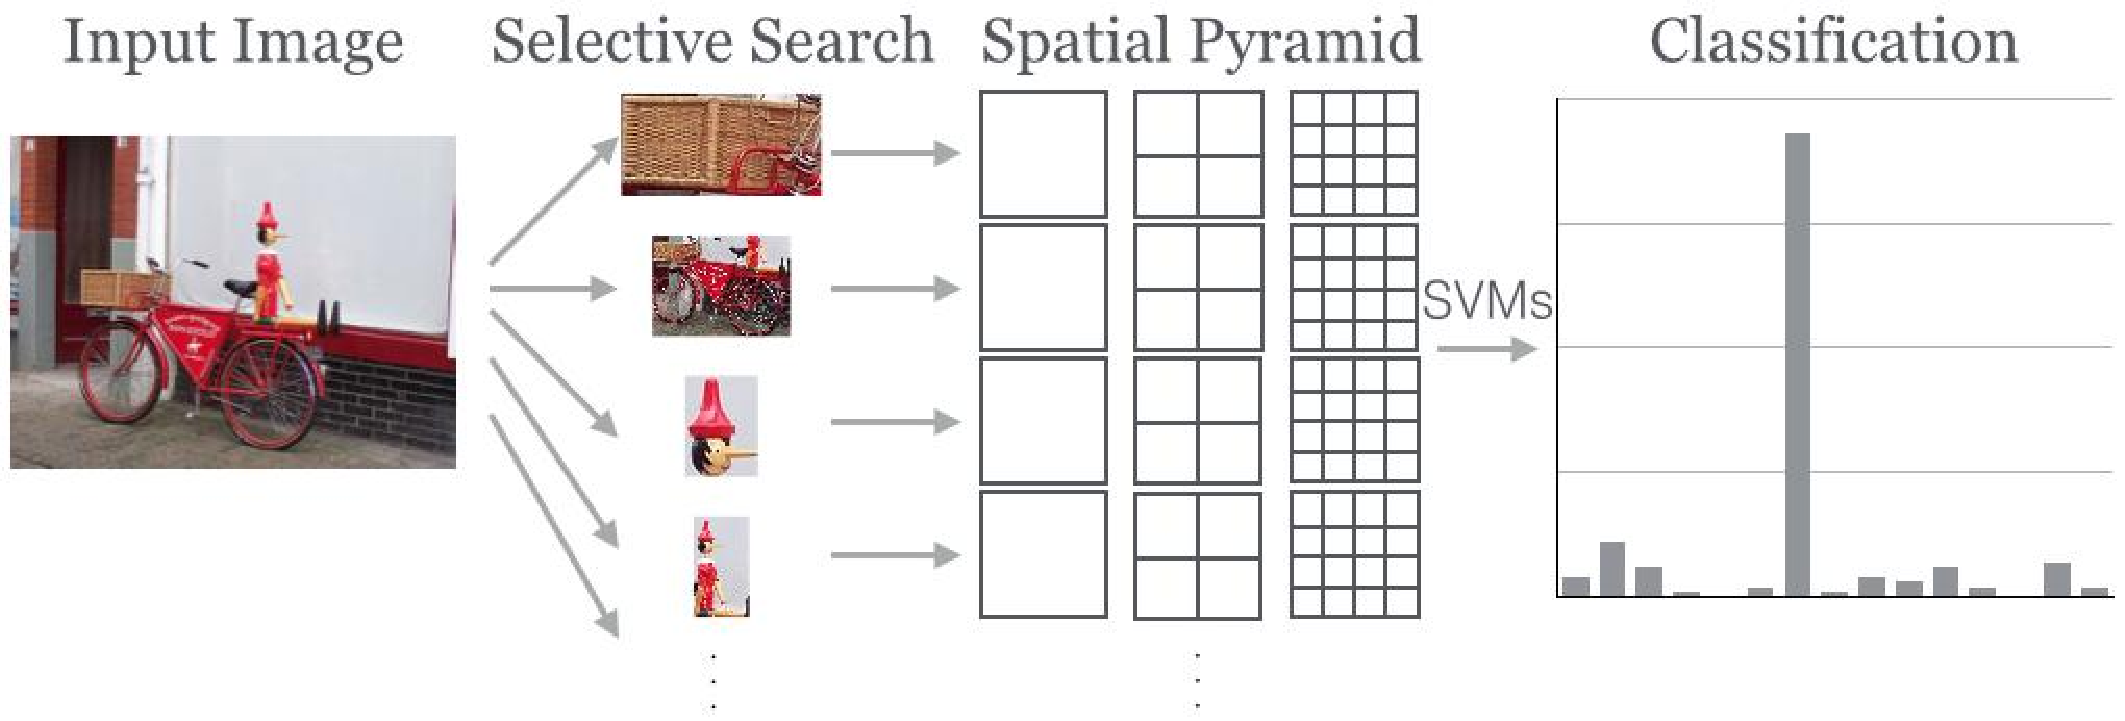
\includegraphics[width=0.8\textwidth]{img/overview.pdf}
  \centering
  \caption{The overview of our system. For an input image, a selective search
  algorithm is applied first to get roughly 2000 regions of interest. We then
  apply a pre-trained Convolutional Neural Network (CNN) on each region of
  interest to get a deep feature vector of length 4096. A three-level spatial
  pyramid representation of the image with deep feature is used to create the
  final feature representation. At each level, for each spatial bin, we use max
  pooling to get the largest feature value of all the feature values of the
  regions of interest which fall into that spatial bin, resulting in the final
  feature of length 4096 $\times$ (1+4+16) as a high-level
  representation of the input image. Then multiple one-vs-all linear SVMs are
  used to do the scene classification.} \label{fig:system_overview}
\end{figure*}

Within this general framework, several methods can be explored to improve the
feature representation. Instead of using the entire image for deep feature
extraction, we can first select a set of region proposals (usually around 2000
for a high-resolution image) which are most informative about the image, then
extract 4096-dimensional feature vectors for each region proposal. This
improvement puts more weights on more informative regions. However, using the
concadenated feature vector would result in an extremely high dimension (2000
$\times$ 4096), it is necessary to use some sparse coding scheme to represent
the global feature pattern. In this paper, we adopt spatial pyramid because of
its simplicity and effectiveness. To increase the generalization ability of our
features and to reduce the impact of overfitting, we further apply $l2$
normalization to the achieved feature vectors before we feed them to the
one-vs-all SVMs. Figure~\ref{fig:system_overview} shows the pipeline of our
system. We will describe the details in the following sections.

\subsection{Generating Region Proposals}
A variety of recent research offers methods for generating category-independent
region proposals for possible object locations. Selective search is one of the
most widely used methods for generating possible object locations for use in
object recognition\cite{Uijlings:2013:SSO}. We argue that same strategy can be
adopted on the indoor scene classification task, because most indoor scenes can
be well characterized by objects they contain. Selective search can exploit
local discriminative information with greatly reduced number of locations
compared to an exhaustive search.  We use selective search to generate region
proposals. Caffe provides a general Python interface for models and it has
a built in interface for selective search. By changing the setting of
``CROP\_MODES'' to ``selective\_search'', we can load the selective search
method to generate roughly 2000 region proposals for an image to feed to the
CNN instead of using an entire image.

\subsection{Feature Extraction}
As we mentioned, we use Caffe, an open source convolutional architecture for
fast feature embedding which contains pre-trained models. Specifically, we use
pre-trained BVLC Reference CaffeNet to extract 4096-dimensional FC 7 feature
vectors from each region proposal. In the Python interface of Caffe, there is
an option to output the features in certain layer rather than only the final
classification results. We set the \textit{blobs} option to \textit{fc7} in
order to obtained FC 7 feature vectors.  The reason to choose FC7 is because it
is the last hidden layer of the CNN, which is supposed to contain the most
informative features. After this step, for one input image, we obtain
a 4096-dimension feature vector for each proposed region.

\subsection{Spatial Pyramid Feature Representation}
The feature vectors created in the previous step has too many dimensions for
both training and prediction. We adopt spatial pyramid matching to generate
a more compact feature vector for an image while still preserve most visual
information in the extracted deep features.  Our spatial pyramid has three
levels, each is generated by equally dividing each rectangular spatial bin of
the previous level into four sub-bins. We generate a single 4096-dimension
feature vector for each spatial bin by max pooling over all the deep features
of the proposed regions that fall in the spatial bin. For three pyramid levels,
there would be $1+4+16$ spatial bins in total, where the first 4096-dimension
feature vector represents the overall visual information of the image, the
following 4$\times$4096-dimension feature vector represents the mid-level
visual information of the image, and the final 16$\times$4096-dimension feature
vector the low-level. We will show the improvement brought by this feature
representation over a simple entire image 4096-dimension feature in
Section~\ref{sec:results}. A $l2$ normalization is followed for better
convergence and less over-fitting.

\subsection{Model Training and Prediction}
Support Vector Machine (SVM) is a useful technique for data classification.
LibSVM\cite{Chang:2011:CC01a} is an integrated software for support vector
classification that is widely used in variety of classification tasks.  It
supports multi-class classification which is used in this project.  We use
libSVM's linear classifier with confidence value option to train 67 one-vs-all
models each for one category in our MIT-indoor67 dataset. During the scene
classification phase, for every testing image, we run the prediction against
all 67 categories and classify the image to the category which has the highest
confidence score.
